\chapter{Variational Autoencoders and Generative Adversarial Net- \\works}

If you remember, the goal of autoencoders was to identify a manifold inside the input space in order to characterize the data. You can think of that of a way to identify the apriori distribution of the data which is the same as we did with the Restricted Boltzmann Machines. In a Restricted Boltzmann Machine once you identified the apriori distribution you can use the model to generate samples that follow the input density. In autoencoders is not as easy to generate new samples. Variational Autoencoders try to solve this so they will be able to both identify the manifold inside the input space and to generate new data according to that probability distribution.

\noindent Variational autoencoders is a type of generative model. Generative models is a model which aim is to learn the apriori probability distribution of the input. So given data with a certain probability distribution $p_{data} (x)$ the goal of a generative model is to learn a probability distribution $p_{model} (x)$ that is as close as possible to the underlying data distribution $p_{data}(x)$. There are two main approaches:

\begin{itemize}
    \item Explicit density estimation. This involves explicitly defining and solving for the probability distribution of the model denoted as $p_{model}(x)$. This is the case for both Boltzmann Machines and Variational Autoencoders. Restricted Boltzmann Machines use an approximation of the density function via Markov Chains (Gibbs sampling) while Variational Autoencoders use an approximation of the density via a variational approach called Evidence Lower Bound (ELBO).
    
    \item Implicit density estimation. This approach consist in learning a model that can sample from $p_{model}(x)$ without explicitly defining it. Generative Adversarial Networks use this approach.
\end{itemize}

\section{Evidence Lower Bound}

In Restricted Boltzmann Machines we have trained our network by maximizing the log-likelihood $log p(v, \theta)$. But because of the partition function is not so easy and we had to use Gibbs sampling to maximize an approximation to this function. For variational autoencoders then we will work with the Evidence Lower Bound that is defined as:

$$L(v, \theta, q) = log p (v, \theta) - D_{KL} \left( q \left( h | v \right) ||  p \left( h | v, \theta \right)  \right) $$

where we subtract from the logarithm of the probability $p(v, \theta)$ the Kullback-Leibler divergence between the conditional probability distribution $p(h | v, \theta)$ and another conditional probability distribution $q(h | v)$, where $q$ is an arbitrary probability distribution over $h$.

\noindent During learning then the goal is to maximize this quantity which means to learn a distribution $q$ that is as similar as possible to $p$. 

\newpage
\noindent Operating on the previous formula:

$$L(v, \theta, q) = log p (v, \theta) - D_{KL} \left( q \left( h | v \right) ||  p \left( h | v, \theta \right)  \right) =  L(v, \theta, q) = log p (v, \theta) - \mathbb{E}_{h\sim q} log \left( \frac{q(h | v)}{p(h | v)}   \right) =$$

$$ log p (v, \theta) - \mathbb{E}_{h\sim q} log \left( \frac{q(h | v)}{\frac{p(h, v, \theta)}{p(v, \theta)}}   \right) = log \left(p (v, \theta) \right) - \mathbb{E}_{h\sim q} \left[ log \left( q(h | v) \right) -  log \left( p(h, v, \theta) \right) + log \left( p(v, \theta) \right)  \right] =$$

$$ L(v, \theta, q) = E_{h \sim q} \left[ log \left(p(h, v) \right) \right] + H(q) $$

where $H(q)$ is the entropy of $q$.

\noindent The idea is then to maximize this equation using a gradient descent algorithm. Since we are working with an expected value we will need to use differentiable generator networks.

\section{Differentiable Generator Networks}

A differentiable generator network are parameterized functions for generating samples. They work by using a differentiable function $g(z, \theta)$ that transforms samples of latent variables $z$ to samples $x$ on the input space (direct approach) or to probability distributions over samples $x$ in the input space (indirect approach). 

These functions $g(z, \theta)$ are typically implemented using a deep neural network where the architecture of the neural network provides the family of possible distributions from which you can sample and the parameters select the specific distribution from within the family.

By generating samples $x$ generator networks allow the definition of a probability distribution $p_g (x)$ and a way to perform Stochastic Gradient Descent of a specific criteria defined on $p_g (x)$ via the reparametrization trick. This trick is used in order to compute the gradient of stochastic transformations of $x$. It consists in augmenting the neural network with an extra set of inputs $z$ that are sample from some simple probability distribution (e.g. $N(0,1)$).

\subsection{Example: Direct Sample Generation}

We can use a direct differentiable generator network to draw samples $x$ from a normal distribution with mean $\mu$ and covariance $\Sigma$. This is done by drawing samples $z$ from a normal distribution with zero mean and identity covariance. Then you feed $z$ to a simple generator network $g$ made of a single affine layer defined as:

$$ x = g(z) = \mu + Lz $$

where $L$ is given by the Cholesky decomposition of $\Sigma$. Being $L^T L = \Sigma$

\subsection{Example: Indirect Sample Generation}

To generate samples in an indirect way, we will define a probability distribution over samples. This is done by using a generator network $g$ with sigmoid outputs to provide the mean parameters of Bernoulli distributions:

$$ p(x_i = 1 \vert z) = g(z)_i $$

\noindent When using the generator network $g$ to define $p(x|z)$, it is possible to impose a distribution over x by marginalizing z:

$$ p(x) =  \sum_z p(x, z) = \sum_z p(z) p(x | z) = \mathbb{E}_z (p(x \vert z))$$

\noindent The generator network then will define a probability distribution $p(x)$ from which we can sample.

\section{Variational Autoencoders}

Given the training dataset $T = \{ x^{(i)} \}_{i=1}^n$ that is known to be generated by a set of latent variables $z$ that we cannot observe. The aim of a Variational Autoencoder is to reproduce this process of generating inputs $x$ given $z$. Basically, this consists on given a variable $z$, sampled from the true apriori probability distribution over the latent space $p_{\theta}(z)$, to sample from the true conditional probability distribution $p_{\theta} (x | z^{(i)})$ in order to generate $x$. To do that, the Variational Autoencoder must estimate the true parameters $\theta$ of this generative model.

\noindent Therefore, first we pick a sample $z$ using a prior distribution probability (e.g. Gaussian). Then we use a generator network for the posterior $p_{\theta} (x)$. Finally instead of maximizing the log-likelihood, we will perform training by maximizing the Evidence Lower Bound.

\noindent This is done because the probability $p_{\theta} (x)$ is intractable.

$$ p_{\theta} (x) = \int p_{\theta}(z) p_{\theta} (x | z) dz $$

\noindent The solution for this is that in addition to the decoder network modelling $p_{\theta}(x|z)$, we define an additional encoder network $q_{\phi} (z | x)$ that approximates $p_{\theta}(x|z)$ using ELBO.

$$ \mathbb{L}(q) = \mathbb{E}_{z \sim q(z \vert x)} \left[ \log (p_{model} (z, x )  ) \right] + H(q(z | x)) = $$  

\noindent Operating we will end up with.

$$ \mathbb{E}_{z \sim q(z \vert x)} \left[ \log (p_{model} (x \vert z)  ) \right] - D_{KL} \left( q( z \vert x) || p_{model} (z)    \right) \leq \log p_{model} (x) $$

Where the Kullback-Leibler divergence forces the encoder $q_{\phi} (z | x)$ to be a Gaussian distribution in order to be able to compute it in a close-form solution. This distribution will act as a prior of $z$. On the other hand, $\mathbb{E}_{z \sim q(z \vert x)} \left[ \log (p_{model} (x \vert z)  ) \right] $ is used to maximize the likelihood of the original input being reconstructed. Notice how $\log (p_{model} (x \vert z) $ defines the decoder and $z \sim q(z \vert x)$ defines the encoder.

\noindent To sum up, the training will consist in finding the $\theta$ and $\phi$ (the parameters for the encoder and decoder respectively) that maximize the lower-bound of the probability distribution of the model.

$$ \theta^*, \phi^* = argmax_{~\theta, \phi} \sum_{i=1}^{N} \mathbb{L} (x^{(i)}, \theta, \phi) $$

\newpage
\noindent This whole process is performed by two Neural Networks one for the encoder and another one for the decoder. So given a set of input data $x$, the encoder is used to return the latent space representations. Once we have that, we will be able to define the latent state distributions with a certain means $\mu$ and variances $\sigma$. Then for the decoder we will sample $z$ from those distributions which will be the input to the decoder network. This network will also define a conditional probability distribution with certain means $\mu$ and variance $\sigma$ in order to generate back the input data $x$.

\begin{figure}[h]
    \centering
    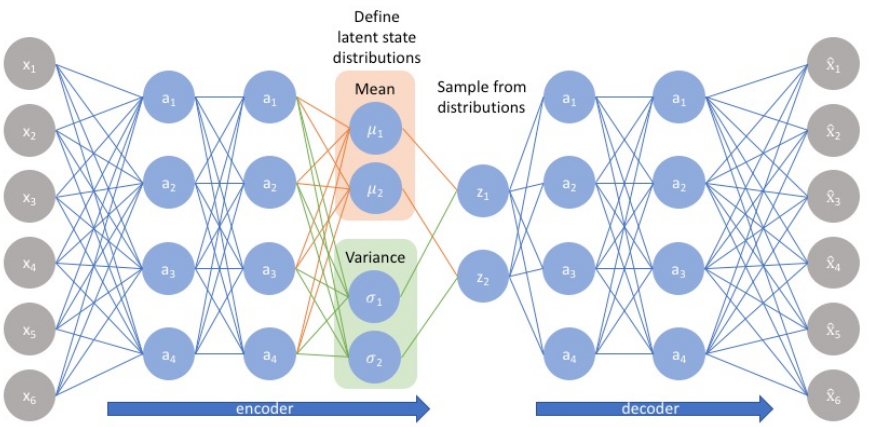
\includegraphics[width=13cm]{Images/vae-architecture.png}
    \caption{Variational Autoencoder architecture}
\end{figure}

\noindent We will be using the reparametrization trick when modelling the sampling of $z$. This is done due to $z \sim q(z | x)$ being a stochastic operator which we are not able to perform gradient descent. Instead, the sampled variable $z$ will be equal to $z = \mu + \sigma \odot \epsilon$ where $\epsilon \sim N(0, 1)$. So instead of sampling from a distribution we are directly generating the sample. 

\begin{figure}[h]
    \centering
    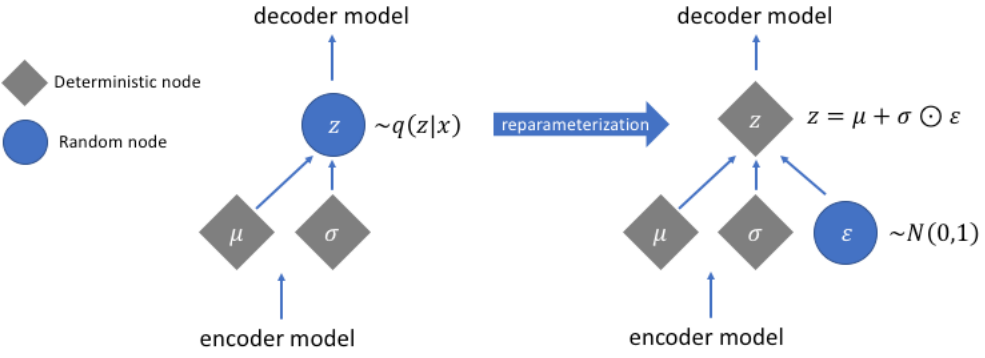
\includegraphics[width=12cm]{Images/reparameterization.png}
    \caption{Reparameterization Trick}
\end{figure}

\newpage
\noindent Once we have trained the whole Variational Autoencoder network we will be able to create new samples given a value $z$ only using the decoder part.

\begin{figure}
    \centering
    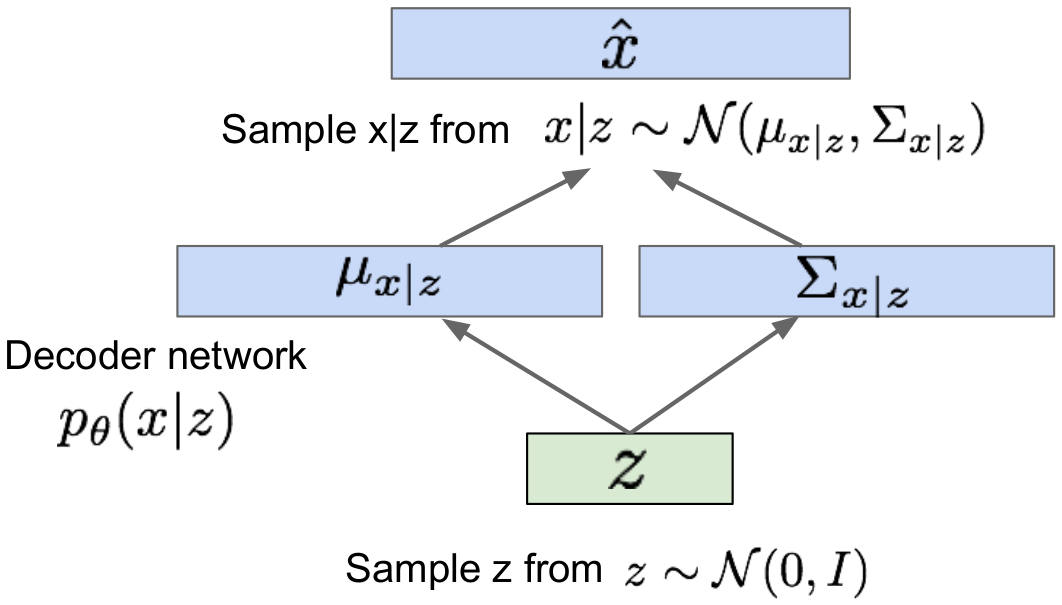
\includegraphics[width=8cm]{Images/decoder-vae.png}
    \caption{VAE decoder architecture for sample generation}
\end{figure}



\newpage
\section{Generative Adversarial Networks}

Generative Adversarial Networks are another generative modeling approach based on differentiable generator networks. In this case they use an indirect approach to generate samples $x$. Instead of learning an explicit probability distribution $p(x)$ to draw samples from, we will be able to generate samples from random noise using a min-max game between a generative and a discriminative network.

Generative Adversarial Networks are based on a game theoretic scenario in which the generator network must compete against an adversary, a discriminative network. The generator network takes a random Gaussian noise input $z$ and transforms it into an output $x=G_{\theta_g} (z)$ that is intended to resemble samples from the training distribution. Meanwhile, its adversary, the discriminator network, attempts to distinguish between samples drawn from the training data and samples drawn from the generator. The discriminator emits a probability value given by $D_{\theta_d} (x)$, indicating the probability that $x$ is a real training example rather than a fake sample drawn from the model.

During the training process, the generator and discriminator networks play a two-player mini-max game. The generator aims to generate samples that the discriminator cannot differentiate from real samples by learning a transformation $G_{\theta_g} (z)$, while the discriminator aims to correctly classify them. As the training progresses, the generator becomes more adept at generating realistic samples, while the discriminator becomes more skilled at distinguishing between real and generated samples.


\begin{figure}[h]
    \centering
    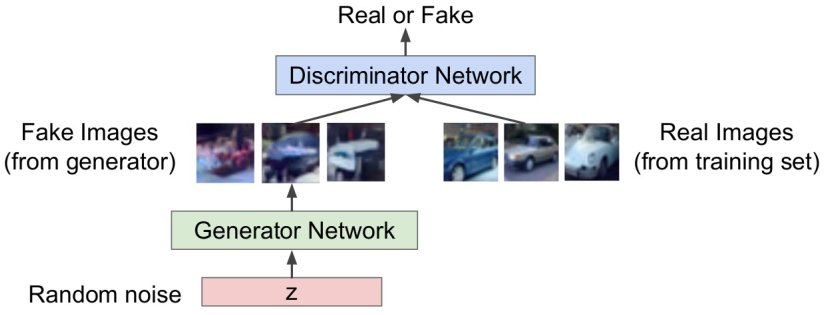
\includegraphics[width=12cm]{Images/gans.jpg}
    \caption{Generative Adversarial Networks schema}
    \label{fig:gans}
\end{figure}

\noindent Through this adversarial process, the generator network gradually learns to transform the random noise input $z$ into samples that resemble the training distribution. The ultimate goal is for the generator network to become so proficient that it can generate high-quality samples that are indistinguishable from real data.

\subsection{Training Generative Adversarial Networks}

In learning we are training jointly by playing a min-max game the objective function:

$$ min_{\theta_g} max_{\theta_d} \left[ \mathbb{E}_{x \sim p_{data}} log D_{\theta_d} (x) + \mathbb{E}_{z \sim p(z)} log \left( 1 - D_{\theta_d} \left( G_{\theta_g} (z)  \right)     \right)    \right] $$

where $D_{\theta_d} (x)$ is the discriminator output for real data $x$ and $D_{\theta_d} \left( G_{\theta_g} (z)  \right)$ is the discriminator output for generated fake data $G(z)$.

\noindent The training procedure is then alternating between performing gradient ascent on the discriminator

$$ max_{\theta_d} \left[ \mathbb{E}_{x \sim p_{data}} log D_{\theta_d} (x) + \mathbb{E}_{z \sim p(z)} log \left( 1 - D_{\theta_d} \left( G_{\theta_g} (z)  \right)     \right)    \right] $$

\noindent and gradient descent in the generative network

$$ min_{\theta_g} \mathbb{E}_{z \sim p(z)} log \left( 1 - D_{\theta_d} \left( G_{\theta_g} (z)  \right)     \right) $$

\noindent If both $G$ and $D$ have enough capacity, and at each step the discriminator $D$ is allowed to reach is optimum given $G$, and the probability distribution of the generative network $p_g$ is updated in order to improve the criteria

$$ max_{\theta_d} \left[ \mathbb{E}_{x \sim p_{data}} log D_{G}^{*} (x) + \mathbb{E}_{x \sim p_g} log \left( 1 - D_{G}^{*} (x)     \right)    \right] $$

then $p_g$ converges to $p_{data}$

\noindent Where for $G$ fixed, the optimal discriminator $D$ is:

$$ D_G^* (x) = \frac{p_{data} (x)}{p_{data} (x) + p_g (x)} $$

\noindent The gradient descent performed on the generator network does not work well in practice. This is because when the sample is likely to be fake, we want to improve the generator. But the gradient in this region is relatively flat. Instead, the gradient signal is strong in the region where the sample is already good. We can change that by maximizing the log-likelihood of the discriminator being wrong which will be performing a gradient ascent in:

$$ max_{\theta_g} \mathbb{E}_{z \sim p(z)} -log \left( D_{\theta_d} \left( G_{\theta_g} (z)  \right)     \right) $$

\begin{figure}[h]
    \centering
    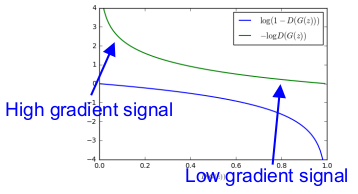
\includegraphics[width=10cm]{Plots/gan-gradient.png}
    \caption{Gradient of the discriminator given the probability that the sample is a a real training sample.}
\end{figure}

\section{Variational Autoencoders vs Generative Adversarial Networks}

Comparing Variational Autoencoders with Generative Adversarial Networks we can see that the training procedure is quite different. Variational Autoencoders are optimized using a variational lower bound on the log-likelihood. Meanwhile, Generative Adversarial Networks use a game theory approach between a discriminative and a generative network.

The advantage of Variational Autoencoders is that they learn a useful latent representation that allows for inference queries. This means learning the probability distribution in the latent explicitly that can be used to generate new samples. Generative Adversarial Networks are not capable of doing that instead is just generate samples using a min-max game with the generative and discriminative networks. Additionally, they can be tricky and unstable to train. 

However, the Generative Adversarial Networks when they are able to converge they generate better samples. The generated samples are usually sharper in contrast with the more smooth or blurred images that the Variational Autoencoder returns.
